\documentclass[12pt]{article}

\usepackage{amsmath,amsthm,amsfonts,amssymb,amsxtra}
\usepackage{pgf,tikz}
\usepackage{multicol}
\usetikzlibrary{arrows}
\renewcommand{\theenumi}{(\alph{enumi})} 
\renewcommand{\labelenumi}{\theenumi}

\pagestyle{empty}
\setlength{\textwidth}{7in}
\setlength{\oddsidemargin}{-0.5in}
\setlength{\topmargin}{-1.0in}
\setlength{\textheight}{9.5in}

\theoremstyle{definition}
\newtheorem{problem}{Problem}

\makeatletter
\newcommand*{\radiobutton}{%
  \@ifstar{\@radiobutton0}{\@radiobutton1}%
}
\newcommand*{\@radiobutton}[1]{%
  \begin{tikzpicture}
    \pgfmathsetlengthmacro\radius{height("X")/2}
    \draw[radius=\radius] circle;
    \ifcase#1 \fill[radius=.6*\radius] circle;\fi
  \end{tikzpicture}%
}
\makeatother

\begin{document}

\noindent{\large\bf MATH 122}\hfill{\large\bf Final Exam}\hfill{\large\bf Fall 2018}\hfill{\large\bf Page 1/6}\hrule

\bigskip
\begin{center}
  \begin{tabular}{|ll|}
    \hline & \cr
    {\bf Name: } & \makebox[12cm]{\hrulefill}\cr & \cr
    {\bf VIP ID:} & \makebox[12cm]{\hrulefill}\cr & \cr
    \hline
  \end{tabular}
\end{center}
\begin{itemize}
\item Write your name and VIP ID in the space provided above.
\item The test has six (6) pages, including this one.
\item Credit for each problem is given in parentheses at the right of the problem number. 
\item You must show sufficient work to justify all answers except on multiple-choice questions.  Correct answers with
  inconsistent or no work will not be given credit.
\item No books or notes may be used on this test.
\item An approved calculator may be used on this test.
\end{itemize}
\hrule

\begin{center}
  \begin{tabular}{|c|c|c|}
    \hline
    &&\cr
    {\large\bf Page} & {\large\bf Max.~points} & {\large\bf Your points} \cr
    &&\cr
    \hline
    &&\cr
    {\Large 2} & \Large 20 & \cr
    &&\cr
    \hline
    &&\cr
    {\Large 3} & \Large 15 & \cr
    &&\cr
    \hline
    &&\cr
    {\Large 4} & \Large 30 & \cr
    &&\cr
    \hline
    &&\cr
    {\Large 5} & \Large 25 & \cr
    &&\cr
    \hline
    &&\cr
    {\Large 6} & \Large 10 & \cr
    &&\cr
    \hline\hline
    &&\cr
    {\large\bf Total} & \Large 100 & \cr
    &&\cr
    \hline
  \end{tabular}
\end{center}

\newpage

%%%%%%%%%%%%%%%%%%%%%%%%%%%%%%%%%%%%% Page 2
\noindent{\large\bf MATH 122}\hfill{\large\bf Final Exam}\hfill{\large\bf Fall 2018}\hfill{\large\bf Page 2/6}\hrule

\bigskip

\begin{problem}[5 pts]
The graph below is a representation of which of the following functions?
\begin{multicols}{2}
\begin{center}
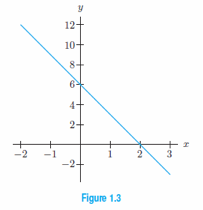
\includegraphics{1graph2.png}
\end{center}
\begin{itemize}
\item[\radiobutton] $y=6x+6$
\item[\radiobutton] $y=-3x+6$
\item[\radiobutton] $y=-3x+2$
\item[\radiobutton] $y=6x-2$
\end{itemize}
\end{multicols}
\end{problem}

\hrule
\begin{problem}[5 pts]
  We are trying to decide between two plumber companies to fix a sink.  The first company charges \$50 for a service
  call, plus an additional \$36 per hour for labor.  The second company charges \$35 for a service call, plus an
  additional \$39 per hour of labor. At how many hours will the two companies charge the same amount of money?

  \vspace{4cm}
\end{problem}
\hrule

\begin{problem}[5 pts each]
Evaluate the following definite integrals.
\begin{enumerate}
\item $\displaystyle{\int_{0}^{4} \ln(y^2 + 1) \, dy} = $
\item $\displaystyle{\int_{10}^{103} 9xe^{30x^2}\, dx = }$
\vspace{7cm}
\end{enumerate}
\end{problem}

\newpage

%%%%%%%%%%%%%%%%%%%%%%%%%%%%%%%%%%%%% Page 3
\noindent{\large\bf MATH 122}\hfill{\large\bf Final Exam}\hfill{\large\bf Fall 2018}\hfill{\large\bf Page 3/6}\hrule

\bigskip

\begin{problem}[5 pts]
If the graph below is that of $f(x)$, which of the following statements is true concerning this function?
\begin{multicols}{2}
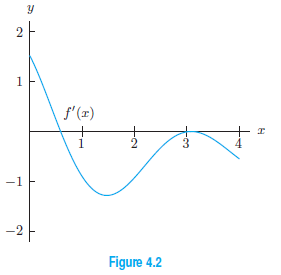
\includegraphics{3graph2}
\vspace{2cm}

\begin{itemize}
\item[\radiobutton] The derivative is zero at two values of $x$, both being local maxima.
\item[\radiobutton] The derivative is zero at two values of $x$, one is a local maximum, while the other is a local minimum.
\item[\radiobutton] The derivative is zero at two values of $x$, one is a local maximum on the interval, while the other is neither a local maximum nor a minimum.
\item[\radiobutton] The derivative is zero at two values of $x$, one is a local minimum on the interval, while the other is neither a local maximum nor a minimum.
\item[\radiobutton] The derivative is zero only at one value of $x$, where it is a local minimum.
\end{itemize}
\end{multicols}
\end{problem}

\hrule
\begin{problem}[5 pts]
Find all local maxima and minima of $f(x) = 2x^3 + 3x^2-180x+9$.
\end{problem}
\vspace{5.5cm}
\hrule
\begin{problem}[5 pts]
Find the global maximum and the global minimum of $f(x) = 2x^3 - 9x^2$ over the interval $-1 \leq x \leq 6$.
\end{problem}

\newpage

%%%%%%%%%%%%%%%%%%%%%%%%%%%%%%%%%%%%% Page 4
\noindent{\large\bf MATH 122}\hfill{\large\bf Final Exam}\hfill{\large\bf Fall 2018}\hfill{\large\bf Page 4/6}\hrule

\bigskip

\bigskip
\begin{problem}[5 pts each]
Find the derivative of the following functions:
\begin{enumerate}
\item $y = 6t^5 - 10\sqrt{t} + \frac{9}{t}$
\begin{flushright}
  \begin{tikzpicture}
    \draw (-4cm,0.5cm) node {$y'(t)=$};
    \draw (-3cm,-0.2cm) rectangle (5cm,1.2cm);
  \end{tikzpicture}
\end{flushright}
\item $f(x) = (2^x + x^5)(3 - \ln x)$
\begin{flushright}
  \begin{tikzpicture}
    \draw (-4cm,0.5cm) node {$f'(x)=$};
    \draw (-3cm,-0.2cm) rectangle (5cm,1.2cm);
  \end{tikzpicture}
\end{flushright}
\item $f(x) = \dfrac{x^8+2}{x}$
\begin{flushright}
  \begin{tikzpicture}
    \draw (-4cm,0.5cm) node {$f'(x)=$};
    \draw (-3cm,-0.2cm) rectangle (5cm,1.2cm);
  \end{tikzpicture}
\end{flushright}
\item $f(x) = \ln \big(8 - e^{-x}\big)$
\begin{flushright}
  \begin{tikzpicture}
    \draw (-4cm,0.5cm) node {$f'(x)=$};
    \draw (-3cm,-0.2cm) rectangle (5cm,1.2cm);
  \end{tikzpicture}
\end{flushright}
\item $f(x) = \big( 6 + \ln x \big)^{0.6}$
\begin{flushright}
  \begin{tikzpicture}
    \draw (-4cm,0.5cm) node {$f'(x)=$};
    \draw (-3cm,-0.2cm) rectangle (5cm,1.2cm);
  \end{tikzpicture}
\end{flushright}
\item $f(x) = 2e^{7x} + e^{-x^6}$
\begin{flushright}
  \begin{tikzpicture}
    \draw (-4cm,0.5cm) node {$f'(x)=$};
    \draw (-3cm,-0.2cm) rectangle (5cm,1.2cm);
  \end{tikzpicture}
\end{flushright}
\end{enumerate}
\end{problem}

\newpage

%%%%%%%%%%%%%%%%%%%%%%%%%%%%%%%%%%%%% Page 5
\noindent{\large\bf MATH 122}\hfill{\large\bf Final Exam}\hfill{\large\bf Fall 2018}\hfill{\large\bf Page 5/6}\hrule

\bigskip 

\begin{problem}[5 pts each]
Compute the antiderivative of the following functions:
\item $\displaystyle{\int x^5 (5 - 3x^6)^{12}\, dx =}$
\vspace{2cm}
\item $\displaystyle{\int  6xe^{x^2} \, dx =}$
\vspace{2cm}
\item $\displaystyle{\int \frac{3x^2}{(8x^3-5)^3} dx =}$
\vspace{4cm}
\item $\displaystyle{\int \frac{dx}{x-4} =}$
\vspace{4cm}
\item $\displaystyle{\int 3x^2 4^{5x^3}\, dx =}$
\end{problem}

\newpage

%%%%%%%%%%%%%%%%%%%%%%%%%%%%%%%%%%%%% Page 6
\noindent{\large\bf MATH 122}\hfill{\large\bf Final Exam}\hfill{\large\bf Fall 2018}\hfill{\large\bf Page 6/6}\hrule

\bigskip  

\begin{problem}[5 pts]
At a price of \$80 for a half-day trip, a white-water rafting company attracts 300 customers.  Every \$5 decrease in price attracts an additional 30 customers.  What price should the company charge per trip to maximize revenue?
\vspace{10cm}
\end{problem}
\hrule

\begin{problem}[5 pts]
The marginal cost of drilling an oil well depends on the depth at which you are drilling; drilling becomes more expensive, per meter, as you dig deeper into the earth.  The fixed costs are one million dollars and, if $x$ is the depth in meters, the marginal costs are $MC(x) = 500 + 12x$ dollars per meter.  Find the \textbf{total cost} of drilling a 400-meter well.
\end{problem}

\end{document}

%%% Local Variables:
%%% mode: latex
%%% TeX-master: t
%%% End:
